\documentclass[xcolor={usenames,dvipsnames}]{beamer}
%
% ugly hack referring to the slides folder. Works for me.
%
\makeatletter
\def\input@path{{/Users/denilson/teaching/cmput391/git-slides/}}
\makeatother

% \usepackage[T1]{fontenc} % font encoding
% \usepackage{fontspec}
\usepackage{fontspec}


\makeatletter%
\@ifclassloaded{beamer}{%
  \usepackage{lmodern} %%% modern beamer style
  %%beamer style
  \usetheme{metropolis}
  \usefonttheme{professionalfonts}
  \setbeamercolor{background canvas}{bg=background}
  \setbeamercolor{frametitle}{bg=snow,fg=black}
  \setbeamercolor{title separator}{fg=snow}
  \setbeamercolor{alerted text}{fg=accent}

  \let\oldtitle\title
  \renewcommand{\title}[1]{\oldtitle{CMPUT391\\#1}}
  \author{Instructor: Denilson Barbosa}
  \date{\small University of Alberta}
  \institute{\today\vskip4em Slides by D. Barbosa, with suggested corrections and improvements by (in alphabetical order) C. Bins, D. Caminhas, K. Guhzva, Q. Lautischer, E. Macdonald, M. A. Nascimento, K. Newbury, M. Strobl, D. Sunderman, K. Wang, and K. Wong.}
  
  \titlegraphic{
\includegraphics[width=1.5cm]{../images/by-sa.png}~
  {\tiny This work is licensed under a Creative Commons Attribution 4.0 International License}}

  %%%% un-framed blocks
  \setbeamertemplate{blocks}[rounded][shadow=false]
}{}

\@ifpackageloaded{xcolor}{}{
  \usepackage{xcolor}
}
\makeatother

\setsansfont[BoldFont={Open Sans SemiBold}]{Open Sans}[Scale=0.9]
\setmonofont{Cousine}[Scale=0.875]
% \setmathtt{Cousine}[Scale=0.875]

%%%% highlighting text 
\usepackage{xspace}
\def\highlight#1{\colorbox{accent}{\textcolor{white}{#1}}\xspace}

\def\blue#1{\textcolor{blue}{#1}}

%
%
%
\usepackage{parskip}

\usepackage{subcaption} % needed for subfigures

\usepackage{wrapfig} % for figures "to the side of the text"

\usepackage{anyfontsize} % for egregious warnings

%
% Fonts
%
% \usepackage{amsmath}
% \usepackage{mathspec}
% \setmathtt[Scale=0.875]{Cousine}

%
% various packages for tables and colored tables
%
\usepackage{xcolor,colortbl}
\usepackage{tcolorbox}

\definecolor{accent}{RGB}{225,68,85}
\definecolor{highlight}{RGB}{170,68,153}
\definecolor{background}{rgb}{253,252,252}

\definecolor{sqlColor}{RGB}{119,119,17}

\definecolor{Cfunction}{RGB}{51,51,153}

\definecolor{stringColor}{RGB}{51,51,153}
\definecolor{datatypeColor}{RGB}{170,68,153}
\definecolor{functionColor}{RGB}{51,134,116}

\definecolor{exampleColor}{RGB}{51,34,136}
\definecolor{commentColor}{RGB}{112,68,225}

\definecolor{fern}{RGB}{80,118,66}

\definecolor{snow}{RGB}{240,240,230}
\definecolor{Gray}{gray}{0.85}

\definecolor{tupleBoxColor}{gray}{0.85}

\definecolor{Maroon}{RGB}{139,0,0}

%
% coloring of SQL code
%
\def\ColorSymbol#1{\textcolor{functionColor}{#1}}

%
% hihglight box
%
\usepackage{xspace}
\def\highlight#1{\colorbox{accent}{\textcolor{white}{#1}}\xspace}

%
% Tables
%
\usepackage{multirow}
\usepackage{multicol}

%
% CODE LISTINGS
%
\usepackage{listings}

%
% catch-all style meant to provide a clean and "empty" style
% from which all others build upon
%
\lstdefinestyle{cmput391}{
  style=,
  frame=no,
  tabsize=2,
  numbers=none,
  showstringspaces=false,
  numberstyle=\footnotesize,
  basicstyle=\ttfamily\footnotesize\color{black},
  numbersep=4pt,
  keywords=[1]{},
  keywords=[2]{},
  keywords=[3]{sh_lock,xl_lock,unlock,read,write,commit,abort},
  keywordstyle=[1]\ttfamily\bfseries\footnotesize,
  keywordstyle=[2]\ttfamily\footnotesize,
  keywordstyle=[3]\ttfamily\footnotesize\color{Maroon},
  emph=[1]{},
  emph=[2]{},
  emph=[3]{},
  emphstyle=[1]\ttfamily\footnotesize,
  emphstyle=[2]\ttfamily\footnotesize,
  emphstyle=[3]\ttfamily\footnotesize,
  commentstyle=\ttfamily\itshape\color{commentColor},
  stringstyle=\ttfamily\color{stringColor},
  moredelim=**[l][\itshape\color{commentColor}]{--},
  moredelim=**[is][\color{highlight}]{-|}{|-},
  moredelim=[is][\bfseries\color{highlight}]{-:}{:-},
  morestring=[s][\color{stringColor}]{"}{"},
  morecomment=[l]{--}
}

\lstdefinelanguage{DTD}{
  style=cmput391,
  morekeywords=[1]{DOCTYPE,ELEMENT,ATTLIST},
  keywordstyle=[1]\color{accent},
  literate = {\#PCDATA}{{\textcolor{Cfunction}{\#PCDATA}}}7
             {\#IMPLIED}{{\textcolor{Cfunction}{\#IMPLIED}}}8
}

\lstdefinelanguage{XPath}{
  style=cmput391,
  morekeywords={xs,integer,current,date,distinct,values,avg,text,id,count,position,and,or,not,boolean,number,sum,floor,ceiling,round,doc,eq,ne,gt,lt,ge,le},
  keywordstyle=\color{red},
  literate = {last(}{{\textcolor{functionColor}{last}(}}5 {@<}{{<}}1  
}

\lstdefinestyle{XQuery}{
  style=cmput391,
  keywords=[1]{if,then,else,and,or,some,every,satisfies,for,in,let,where,group,order,by,return,ascending},
  keywords=[2]{gt,lt,eq,ne,ge,le,not,or},
  keywords=[3]{text,sum,min,max,avg,len,position,number,boolean,floor,ceiling,round,%
               id,doc,count,current-date,distinct-values,xs:integer,subsequence},
  keywordstyle=[1]\bfseries\color{sqlColor},
  keywordstyle=[2]\color{accent},
  keywordstyle=[3]\color{functionColor},
  moredelim =[is][\color{blue}]{-:}{:-},
  moredelim =[s][\color{accent}]{<}{>},
  moredelim=**[s][\color{black}]{/}{\ },
  moredelim=*[s][\color{blue}]{\$}{\ },
  alsoletter=:{:,-},
  literate = {(}{{\textcolor{black}{(}}}{1} {)}{{\textcolor{black}{)}}}{1} 
             {\{}{{\textcolor{black}{\{}}}{1} {\}}{{\textcolor{black}{\}}}}{1} 
             {last(}{{\textcolor{functionColor}{last}(}}5 {@<}{{<}}1
}


\lstdefinestyle{SQL}{
  style=cmput391,
  language=SQL,
  sensitive={True},
  deletekeywords={year,Cast,MIN,MAX},
  morekeywords={ABORT,AFTER,BEFORE,REFERENCES,REFERENCING,WITH,COMMITTED,UNCOMMITTED,REPEATABLE,SERIALIZABLE},
  keywords=[2]{AVG,MIN,MAX,COUNT,SUM,NEW,OLD,strftime,date,length,RAISE,rowid,substr},
  keywords=[3]{BIGINT,CHAR,DATE,DECIMAL,INT,FLOAT,TEXT},
  keywordstyle=[1]\ttfamily\bfseries\color{sqlColor},
  keywordstyle=[2]\ttfamily\bfseries\color{functionColor},
  keywordstyle=[3]\ttfamily\bfseries\color{datatypeColor},
  moredelim=**[is][\ttfamily\bfseries\color{functionColor}]{(@}{@)},
  morestring=[s][\color{stringColor}]{'}{'},
  moredelim=[is][\bfseries\color{highlight}]{-:}{:-}
}


%
% lstlisting for command line examples
%
\lstdefinestyle{commandLine}{
  basicstyle=cmput391,
  keywordstyle=[1]\ttfamily\bfseries\color{functionColor},
  keywordstyle=[2]\ttfamily\bfseries\color{datatypeColor},
  moredelim=**[is][\color{accent}\bf]{@}{@}
  keywords=[1]{%
    grep},
  keywords=[2]{%
    postings}
}

%
% lstlisting for C code
%
\lstdefinestyle{C}{
  language=C,
  tabsize=2,
  basicstyle=\ttfamily\footnotesize,
  stringstyle=\color{stringColor},
  keywords=[2]{sqlite3_prepare_v2,sqlite3_bind_int64,sqlite3_step,sqlite3_exec},
  keywordstyle=[1]\ttfamily\bfseries\color{datatypeColor},
  keywordstyle=[2]\ttfamily\bfseries\color{functionColor},
  commentstyle=\ttfamily\itshape\color{commentColor},
  moredelim=**[is][\color{Cfunction}\bf\ttfamily]{@}{@}
}


\lstdefinestyle{Python}{
  language=Python,
  tabsize=2,
  basicstyle=\ttfamily\footnotesize,
  stringstyle=\color{stringColor},
  morekeywords=[1]{self,yield,Class,true,false,None},
  keywords=[2]{satisfies,from,Iterator,EOF,concatenate,advance,join,rewind},
  deletekeywords=[1]{from},
  keywordstyle=[1]\ttfamily\bfseries\color{datatypeColor},
  keywordstyle=[2]\ttfamily\bfseries\color{functionColor},
  commentstyle=\ttfamily\itshape\color{commentColor},
  moredelim=**[is][\color{Cfunction}\bf\ttfamily]{@}{@}
}



%
% lstlisting style for RDF/SPARQL
%
\lstdefinestyle{SPARQL}{
  style=cmput391,
  sensitive={True},
  keywords=[1]{BASE,PREFIX,SELECT,WHERE,FILTER,MINUS,NOT,EXISTS},
  keywordstyle=[1]\ttfamily\bfseries\color{sqlColor},
  moredelim=*[s][\color{Cfunction}]{?}{\ },
  moredelim=*[s][\color{Cfunction}]{@}{\ },
  morestring=[s][\color{datatypeColor}]{"}{"},
  literate =* {|}{{|}}1 {//}{{//}}2 {< }{< }{2}
}

%
% coloring of markup code
%
\lstdefinestyle{markup}{
  style=cmput391,
  literate =* {=}{{\color{sqlColor}{=}}}1,
  moredelim =* [s][\color{accent}]{<}{>},
  moredelim =** [is][\color{accent}]{@}{@},
  moredelim =** [is][\color{blue}]{-:}{:-},
  morecomment=[s]{<!--}{-->}
}

\lstdefinestyle{RDF}{
  style=cmput391,
  keywords=[1]{BASE,PREFIX},
  keywordstyle=[1]\ttfamily\bfseries\color{functionColor},
  alsoletter=:{:,-,@},
  literate = {prefix}{{\bfseries\textcolor{functionColor}{prefix}}}6 
             {:}{{\textcolor{functionColor}{:}}}1 
             {@}{{\textcolor{functionColor}{@}}}1,
  moredelim =* [s][\color{accent}]{<}{>},
  moredelim =** [is][\color{functionColor}]{-:}{:-},
  morecomment=[s]{<!--}{-->}
}




















%
% Tikz stuff, for cummulative diagrams and algebra trees
%
\usepackage{tikz} %commutative diagrams
\usepackage{tikz-cd} %commutative diagrams
\usetikzlibrary{positioning}% To get more advances positioning options
\usetikzlibrary{arrows,shapes,automata}
\usetikzlibrary{calc} % for calculations and hard-coded coordinates
\usetikzlibrary{tikzmark, fit, shapes.misc}
\usetikzlibrary{decorations.pathreplacing}
\usetikzlibrary{backgrounds} % to draw underneath other elements
\usepackage{stackengine} % to overlay tikz pictures over other things

\usepackage{pgfplots}
\pgfplotsset{compat=1.17}

%
%
% PGF arrowtip that looks like an X
%
%
\pgfarrowsdeclare{X}{X}
{
  \arrowsize=0.25pt
  \advance\arrowsize by .5\pgflinewidth
  \pgfarrowsleftextend{-4\arrowsize-.5\pgflinewidth}
  \pgfarrowsrightextend{.5\pgflinewidth}
}
{
  \arrowsize=0.2pt
  \advance\arrowsize by .5\pgflinewidth
  \pgfsetdash{}{0pt} % do not dash
  \pgfsetroundjoin   % fix join
  \pgfsetroundcap    % fix cap
  \pgfpathmoveto{\pgfpointorigin}
  \pgfpathlineto{\pgfpoint{-5\arrowsize}{5\arrowsize}}
  \pgfusepathqstroke
  \pgfpathmoveto{\pgfpointorigin}
  \pgfpathlineto{\pgfpoint{5\arrowsize}{-5\arrowsize}}
  \pgfusepathqstroke
  \pgfpathmoveto{\pgfpointorigin}
  \pgfpathlineto{\pgfpoint{-5\arrowsize}{-5\arrowsize}}
  \pgfusepathqstroke
  \pgfpathmoveto{\pgfpointorigin}
  \pgfpathlineto{\pgfpoint{5\arrowsize}{5\arrowsize}}
  \pgfusepathqstroke
}


%
%%% for algorithms and pseudocode
%
\usepackage{algorithm}
% \usepackage{algpseudocode}
\usepackage[noend]{algpseudocode}
\renewcommand{\algorithmicrequire}{\textbf{Input:}}
\renewcommand{\algorithmicensure}{\textbf{Output:}}
\algnewcommand\algorithmicforeach{\textbf{for each}}
\algdef{S}[FOR]{ForEach}[1]{\algorithmicforeach\ #1\ \algorithmicdo}
% style for comments inside algorithms
\renewcommand{\algorithmiccomment}[1]{\hspace*{1em}\textcolor{commentColor}{\%~\textit{#1}}} 

%
% to create boxes with verbatim and code-like content
%
\usepackage{verbatimbox}

%
% to crop/trim boxes!
%
\usepackage{trimclip}

%
% colored and framed boxes
%
\newenvironment{BOX}[1]{\begin{tcolorbox}[colback=snow!25,colframe=snow!40!black,title=#1]\small}{\end{tcolorbox}}



%
% math and symbols
%
\usepackage{mathtools}
\DeclarePairedDelimiter{\ceil}{\lceil}{\rceil}
\DeclarePairedDelimiter{\floor}{\lfloor}{\rfloor}
\usepackage{amsbsy} 
\usepackage{amssymb}
\usepackage{ifsym} % needed to produce the common outerjoin symbols

%
% for nice-looking enumerations and inlined enumerations
%
\usepackage[shortlabels,inline]{enumitem}



%%% outer join symbols
\newcommand\TextbookOuterJoin{%
  \mathrel{\ooalign{\hss$\Join$\hss\cr%
  \kern0.5ex\raise1ex\hbox{\scalebox{0.7}{$\circ$}}}}}

\newcommand\RightOuterJoin{%
  \mathrel{%
  	\ooalign{%
  		$\Join$\cr\kern1.25ex\raise0.0975ex\hbox{\scalebox{0.25}[0.8275]{$\sqsubset$}}}
  	}
}

\newcommand\LeftOuterJoin{%
  \mathrel{%
  	\ooalign{%
  		$\Join$\cr\kern-0.0125ex\raise0.0975ex\hbox{\scalebox{0.25}[0.8275]{$\sqsupset$}}}%
	}
}

\newcommand\FullOuterJoin{%
  \mathrel{%
  	\ooalign{%
  		$\Join$\cr\kern-0.0125ex\raise0.0975ex\hbox{\scalebox{0.25}[0.8275]{$\sqsupset$}}}%
  		\kern-0.45ex\raise0.0975ex\hbox{\scalebox{0.25}[0.8275]{$\sqsubset$}}
	}
}






\title{Intro to CMPUT 391}

\begin{document}


% full relational schema

\newsavebox\FullMovieSchema
\begin{lrbox}{\FullMovieSchema}\begin{minipage}{\textwidth}
\begin{lstlisting}[style=SQL]
CREATE TABLE Movie (title CHAR(20), year INT, imdb FLOAT,
   PRIMARY KEY (title, year), CHECK(imdb >= 0 AND imdb <= 10));
CREATE TABLE Director (name CHAR(20), PRIMARY KEY (name));
CREATE TABLE Actor (name CHAR(20), PRIMARY KEY (name));
CREATE TABLE Cinema (name CHAR(20), address CHAR(100), 
   PRIMARY KEY(name));

CREATE TABLE MovieDirector (title CHAR(20), year INT, name CHAR(20)
  PRIMARY KEY (title, year, name),
  FOREIGN KEY (title, year) REFERENCES Movie(title, year),
  FOREIGN KEY (name) REFERENCES Director(name));

CREATE TABLE Cast (title CHAR(20), year INT, name CHAR(20), role CHAR(20), 
  PRIMARY KEY (title, year, name, role),
  FOREIGN KEY (title, year) REFERENCES Movie(title, year)
  FOREIGN KEY (name) REFERENCES Actor(name));

CREATE TABLE Guide (theater CHAR(20), film CHAR(20), year INT, start INT, 
  PRIMARY KEY (theater, film, year, start),
  FOREIGN KEY (theater) REFERENCES Cinema(name), 
  FOREIGN KEY (film, year) REFERENCES Movie(title, year));
\end{lstlisting}
\end{minipage}
\end{lrbox}


% simplified relational schema

\newsavebox\SimplifiedMovieSchema
\begin{lrbox}{\SimplifiedMovieSchema}\begin{minipage}{\textwidth}
\begin{lstlisting}[style=SQL]
CREATE TABLE Movie (title CHAR(20), year INT, imdb FLOAT, 
   director CHAR(20) NOT NULL, PRIMARY KEY (title, year), 
   CHECK(imdb >= 0 AND imdb <= 10));

CREATE TABLE Cinema (name CHAR(20), address CHAR(100), 
   PRIMARY KEY(name));

CREATE TABLE Cast (title CHAR(20), year INT, 
   actor CHAR(20) NOT NULL, role CHAR(20) NOT NULL, 
   FOREIGN KEY (title, year) REFERENCES Movie(title, year));

CREATE TABLE Guide (theater CHAR(20), film CHAR(20), year INT, start INT, 
  PRIMARY KEY (theater, film, year, start),
  FOREIGN KEY (theater) REFERENCES Cinema(name), 
  FOREIGN KEY (film, year) REFERENCES Movie(title, year));
\end{lstlisting}
\end{minipage}
\end{lrbox}

% simplified CREATE MOVIE example

\newsavebox\SimplifiedMovieTableDDL
\begin{lrbox}{\SimplifiedMovieTableDDL}\begin{minipage}{0.9\textwidth}
\begin{lstlisting}[style=SQL]
CREATE TABLE Movie (title CHAR(20), year INT, imdb FLOAT, 
   director CHAR(20), PRIMARY KEY (title, year), 
   CHECK(imdb >= 0 AND imdb <= 10));
\end{lstlisting}
\end{minipage}
\end{lrbox}

% simplified CREATE CAST example

\newsavebox\SimplifiedCastTableDDL
\begin{lrbox}{\SimplifiedCastTableDDL}\begin{minipage}{\textwidth}
\begin{lstlisting}[style=SQL]
CREATE TABLE Cast (title CHAR(20), year INT, 
   actor CHAR(20), role CHAR(20), 
   FOREIGN KEY (title, year) REFERENCES Movie(title, year);
\end{lstlisting}
\end{minipage}
\end{lrbox}
%
% this file has latex "boxes" with each of the tables
% and query results for the examples involving the
% movies database
%

\newsavebox{\MovieTable}
\savebox{\MovieTable}{%
\scriptsize%
\begin{tabular}{l | l | c | l }
\multicolumn{4}{l}{\textbf{Movie}}\\
\hline
\rowcolor{Gray}
\textbf{title} & \textbf{year} & \textbf{imdb} & \textbf{director} \\
\hline
Ghostbusters & 1984 & 7.8 & Ivan Reitman \\
\hline
Big & 1988 & 7.3 & Penny Marshall \\
\hline
Lost in Translation & 2003 & 7.8 & Sofia Coppola \\
\hline
Wadjda & 2012 & 8.1 & Haifaa al-Mansour \\
\hline
Ghostbusters & 2016 & 5.3 & Paul Feig \\
\hline
\end{tabular}
}

\newsavebox{\MovieTableTWO}
\savebox{\MovieTableTWO}{%
\scriptsize%
\begin{tabular}{l | l | c | l }
\multicolumn{4}{l}{\textbf{Movie}}\\
\hline
\rowcolor{Gray}
\textbf{title} & \textbf{year} & \textbf{imdb} & \textbf{director} \\
\hline
Lost in Translation & 2003 & 7.8 & Haifaa al-Mansour \\ % fake tuple :)
\hline
Groundhog day & 1993 & 8 & Harold Ramis \\
\hline
\end{tabular}
}


\newsavebox{\CinemaTable}
\savebox{\CinemaTable}{%
\scriptsize%
\begin{tabular}{l | l }
\multicolumn{2}{l}{\textbf{Cinema}}\\
\hline
\rowcolor{Gray}
\textbf{name} & \textbf{address}  \\
\hline
Garneau & 8712 109 St, Edmonton \\
\hline
Princess & 10337 82 Ave, Edmonton \\
\hline
Landmark & 10200 102 Ave, Edmonton\\
\hline
\end{tabular}
}

\newsavebox{\GuideTable}
\savebox{\GuideTable}{%
\scriptsize%
\begin{tabular}{l | l | l | l }
\multicolumn{4}{l}{\textbf{Guide}}\\
\hline
\rowcolor{Gray}
\textbf{theater} & \textbf{film} & \textbf{year} & \textbf{start}  \\
\hline
Garneau & Ghostbusters & 1984 & 1140 \\
\hline
Garneau & Ghostbusters & 2016 & 1290 \\
\hline
Princess & Wadjda & 2012 & 1260 \\
\hline
\end{tabular}
}


\newsavebox{\CastTable}
\savebox{\CastTable}{%
\scriptsize%
\begin{tabular}{l | l | l | l }
\multicolumn{4}{l}{\textbf{Cast}}\\
\hline
\rowcolor{Gray}
\textbf{title} & \textbf{year} & \textbf{actor} & \textbf{role}  \\
\hline
Ghostbusters & 1984 & Bill Murray & Dr. Venkman \\
\hline
Ghostbusters & 1984 & Sigourney Weaver & Dana Barret \\
\hline
Big & 1988 & Tom Hanks & Josh \\
\hline
Big & 1988 & Elisabeth Perkins & Susan \\
\hline
Lost in Translation & 2003 & Bill Murray & Bob Harris \\
\hline
Wadjda & 2012 & Waad Mohammed & Wadjda \\
\hline
Ghostbusters & 2016 & Dan Aykroyd & Cabbie \\
\hline
Ghostbusters & 2016 & Sigourney Weaver & Dana Barret \\
\hline
\end{tabular}
}

%
% box with all tables together.
%
%%%% NEED TO FIND A NICER WAY THAN THIS...
\newsavebox{\FullInstance}
\savebox{\FullInstance}{%
	\begin{tabular}{@{}l@{}}
		\resizebox{0.6\textwidth}{!}{\usebox{\MovieTable}}\\
		~\\[-0.5em]
		\resizebox{0.7\textwidth}{!}{\usebox{\CastTable}}\\
		~\\[-0.5em]
		\resizebox{0.95\textwidth}{!}{\usebox{\CinemaTable}~~~\usebox{\GuideTable}
		}%
	\end{tabular}%
}

%
% example movie column-oriented store
%
\newsavebox{\MovieTableColTitle}
\savebox{\MovieTableColTitle}{%
\scriptsize%
\begin{tabular}{l | l}
\hline
\rowcolor{Gray}
\ColorSymbol{\textbf{id}} &\textbf{title} \\
\hline
\ColorSymbol{1} & Ghostbusters \\
\hline
\ColorSymbol{2} & Big \\
\hline
\ColorSymbol{3} & Lost in Translation \\
\hline
\ColorSymbol{4} & Wadjda \\
\hline
\ColorSymbol{5} & Ghostbusters \\
\hline
\end{tabular}
}

\newsavebox{\MovieTableColYear}
\savebox{\MovieTableColYear}{%
\scriptsize%
\begin{tabular}{l | l }
\hline
\rowcolor{Gray}
\ColorSymbol{\textbf{id}} &\textbf{year} \\
\hline
\ColorSymbol{1} & 1984 \\
\hline
\ColorSymbol{2} & 1988 \\
\hline
\ColorSymbol{3} & 2003 \\
\hline
\ColorSymbol{4} & 2012 \\
\hline
\ColorSymbol{5} & 2016 \\
\hline
\end{tabular}
}

\newsavebox{\MovieTableColIMDB}
\savebox{\MovieTableColIMDB}{%
\scriptsize%
\begin{tabular}{l | l}
\hline
\rowcolor{Gray}
\ColorSymbol{\textbf{id}} &\textbf{imdb} \\
\hline
\ColorSymbol{1} & 7.8 \\
\hline
\ColorSymbol{2} & 7.3 \\
\hline
\ColorSymbol{3} & 7.8 \\
\hline
\ColorSymbol{4} & 8.1 \\
\hline
\ColorSymbol{5} & 5.3 \\
\hline
\end{tabular}
}

\newsavebox{\MovieTableColDirector}
\savebox{\MovieTableColDirector}{%
\scriptsize%
\begin{tabular}{l | l}
\hline
\rowcolor{Gray}
\ColorSymbol{\textbf{id}} &\textbf{director} \\
\hline
\ColorSymbol{1} & Ivan Reitman \\
\hline
\ColorSymbol{2} & Penny Marshall \\
\hline
\ColorSymbol{3} & Sofia Coppola \\
\hline
\ColorSymbol{4} & Haifaa al-Mansour  \\
\hline
\ColorSymbol{5} & Paul Feig \\
\hline
\end{tabular}
}


%
% Table with selection on Cast.actor='Bill Murray'
%
\newsavebox{\BillMurrayMovies}
\savebox{\BillMurrayMovies}{%
\scriptsize%
\begin{tabular}{l | l | l | l }
\rowcolor{Gray}
\hline
\textbf{title} & \textbf{year} & \textbf{actor} & \textbf{role}  \\
\hline
Ghostbusters & 1984 & Bill Murray & Dr. Venkman \\
\hline
Lost in Translation & 2003 & Bill Murray & Bob Harris \\
\hline
\end{tabular}
}

%
% Table with projection of director on Movie
%
\newsavebox{\MovieDirectors}
\savebox{\MovieDirectors}{%
\scriptsize%
\begin{tabular}{l }
\rowcolor{Gray}
\hline
\textbf{director}  \\
\hline
Ivan Reitman \\
\hline
Penny Marshall \\
\hline
Sofia Coppola \\
\hline
Haifaa al-Mansour  \\
\hline
Paul Feig \\
\hline
\end{tabular}
}

%
% Table with Movie \bowtie \sigma Cast.actor='Bill Murray'
%
\newsavebox{\JoinMoviesBillMurrayMovies}
\savebox{\JoinMoviesBillMurrayMovies}{%
\scriptsize%
\begin{tabular}{l | l | c | l | l | l }
\rowcolor{Gray}
\hline
\textbf{title} & \textbf{year} & \textbf{imdb} & \textbf{director} & \textbf{actor} & \textbf{role}  \\
\hline
Ghostbusters & 1984 & 7.8 & Ivan Reitman & Bill Murray & Dr. Venkman \\
\hline
Lost in Translation & 2003 & 7.8 & Sofia Coppola & Bill Murray & Bob Harris \\
\hline
\end{tabular}
}

%
% Left Outer Join of Cinema and Guide
%
\newsavebox{\LeftOuterJoinCinemaGuide}
\savebox{\LeftOuterJoinCinemaGuide}{%
\scriptsize%
\begin{tabular}{l | l | l | l | l | l}
\hline
\rowcolor{Gray}
\textbf{name} & \textbf{address} & \textbf{theater} & \textbf{film} & \textbf{year} & \textbf{start} \\
\hline
Garneau & 8712 109 St, Edmonton & Garneau & Ghostbusters & 1984 & 1140 \\
\hline
Garneau & 8712 109 St, Edmonton & Garneau & Ghostbusters & 2016 & 1290 \\
\hline
Princess & 10337 82 Ave, Edmonton & Princess & Wadjda & 2012 & 1260 \\
\hline
Landmark & 10200 102 Ave, Edmonton & NULL & NULL & NULL & NULL\\
\hline
\end{tabular}
}

%
% Semijoin of Cinema and Guide
%
\newsavebox{\SemijoinCinemaGuide}
\savebox{\SemijoinCinemaGuide}{%
\scriptsize%
\begin{tabular}{l | l }
\hline
\rowcolor{Gray}
\textbf{name} & \textbf{address}  \\
\hline
Garneau & 8712 109 St, Edmonton \\
\hline
Princess & 10337 82 Ave, Edmonton \\
\hline
\end{tabular}
}

%
% Single tuple in self-join of Cast to get actors in reruns
%
\newsavebox{\SelfJoinExampleSigourneyWeaver}
\savebox{\SelfJoinExampleSigourneyWeaver}{%
\scriptsize%
\begin{tabular}{l | l | l | l | l | l | l | l}
\hline
\rowcolor{Gray}
\textbf{title} & \textbf{year} & \textbf{actor} & \textbf{role}  & \textbf{title2} & \textbf{year2} & \textbf{actor2} & \textbf{role2} \\
\hline
Ghostbusters & 1984 & Sigourney Weaver & Dana Barret & Ghostbusters & 2016 & Sigourney Weaver & Dana Barret \\
\hline
\end{tabular}
}

%
% result of select theater, count(*) on Guide
%
\newsavebox{\CountStartOnGuideTable}
\savebox{\CountStartOnGuideTable}{%
\scriptsize%
\begin{tabular}{l | l }
\hline
\rowcolor{Gray}
\textbf{theater} & \textbf{COUNT} \\
\hline
Garneau & 2\\
\hline
Princess & 1\\
\hline
\end{tabular}
}

% ---------------------- get the tuplex from the example tables

\newsavebox\MovieI
\savebox{\MovieI}{
	\clipbox{0 45.125 0 22.125}{\usebox\MovieTable}
}
\newsavebox\MovieII
\savebox{\MovieII}{
	\clipbox{0 33.75 0 33.45}{\usebox\MovieTable}
}
\newsavebox\MovieIII
\savebox{\MovieIII}{
	\clipbox{0 22.65 0 44.75}{\usebox\MovieTable}
}
\newsavebox\MovieIV
\savebox{\MovieIV}{
	\clipbox{0 11.3 0 56}{\usebox\MovieTable}
}
\newsavebox\MovieV
\savebox{\MovieV}{
	\clipbox{0 0 0 67.25}{\usebox\MovieTable}
}

\newsavebox\MovieVI
\savebox{\MovieVI}{
	\clipbox{0 0 0 33.5}{\usebox\MovieTableTWO}
}

\def\movieTupleGHOSTBUSTERSone{\scalebox{0.75}{\usebox{\MovieI}}}
\def\movieTupleBIG{\scalebox{0.75}{\usebox{\MovieII}}}
\def\movieTupleLOSTinTRANSLATION{\scalebox{0.75}{\usebox{\MovieIII}}}
\def\movieTupleWADJDA{\scalebox{0.75}{\usebox{\MovieIV}}}
\def\movieTupleGHOSTBUSTERStwo{\scalebox{0.75}{\usebox{\MovieV}}}
\def\movieTupleGROUNDHOGday{\scalebox{0.75}{\usebox{\MovieVI}}}

\def\idxKeyTitleBIG{\scalebox{0.75}{\clipbox{5 0 140 0}{\usebox\MovieII}}}
\def\idxKeyTitleGHOSTBUSTERSone{\scalebox{0.75}{\clipbox{5 0 140 0}{\usebox\MovieI}}}
\def\idxKeyTitleGHOSTBUSTERStwo{\scalebox{0.75}{\clipbox{5 0 140 0}{\usebox\MovieV}}}
\def\idxKeyTitleLOSTinTRANSLATION{\scalebox{0.75}{\clipbox{5 0 140 0}{\usebox\MovieIII}}}
\def\idxKeyTitleWADJDA{\scalebox{0.75}{\clipbox{5 0 140 0}{\usebox\MovieIV}}}

\def\idxKeyTitleYearBIG{\scalebox{0.75}{\clipbox{8 0 111 0}{\usebox\MovieII}}}
\def\idxKeyTitleYearGHOSTBUSTERSone{\scalebox{0.75}{\clipbox{8 0 111 0}{\usebox\MovieI}}}
\def\idxKeyTitleYearGHOSTBUSTERStwo{\scalebox{0.75}{\clipbox{8 0 111 0}{\usebox\MovieV}}}
\def\idxKeyTitleYearLOSTinTRANSLATION{\scalebox{0.75}{\clipbox{8 0 111 0}{\usebox\MovieIII}}}
\def\idxKeyTitleYearWADJDA{\scalebox{0.75}{\clipbox{8 0 111 0}{\usebox\MovieIV}}}


% -------------------------- macros for drawing tuples in the data file

\tikzset{
	tuple/.style={
		anchor=north west,
		inner sep=0pt,outer sep=0pt,shift={(0pt,-2pt)}
	}
}

\tikzset{ % same as above, except for the anchor part
	tupleBelow/.style={
		inner sep=0pt,outer sep=0pt,shift={(0pt,-2pt)}
	}
}


% #1     --> id of tuple (i.e., the node with the value)
% #2, #3 --> coordinages of top-left corner of node with tuple value
% #4     --> value in the attribute of the tuple
\def\tuple#1#2#3#4{
  \node ({#1}) at ({#2},{#3}) [tuple] {{#4}} ;
}

% #1     --> id of tuple (i.e., the node with the value)
% #2, #3 --> coordinages of top-left corner of node with tuple value
% #4     --> value in the attribute of the tuple
\def\tupleBelow#1#2#3{
  \node ({#1}) [below = -2pt of {#2}] [tupleBelow] {{#3}} ;
}


% --------------------------- macros for drawing blocks of the data file

\tikzset{
	MovieDataBlock/.style={
		draw,rectangle,minimum width=5.5125cm, minimum height=0.69cm,anchor=north west,inner sep=1pt,outer sep=1pt
	}
}

\tikzset{
	MovieDataBlockPointerBox/.style={
		fill=snow,draw,rectangle,minimum width=1em,minimum height=1em,
		anchor=north west,
		inner sep=1pt,outer sep=1pt,
		shift={(5.5125cm,-0.34cm)}
	}
}


% #1    --> block id
% #2,#3 --> coordinates of top-left corner
% #4    --> id of the first tuple
% #5    --> value of the first tuple
\def\movieDataBlock#1#2#3#4#5{
	\node ({#1}) at ({#2},{#3}) [MovieDataBlock] {};
	\node at ({#2},{#3}) [MovieDataBlockPointerBox] {};
	
	\tuple{#4}{#2}{#3}{#5};
}

% #1     --> block id
% #2     --> id of block ``above'' this one
% #3, #4 --> coordinates of this block
% #5     --> id of the first tuple inside the block
% #6     --> value of the first tuple
\def\movieDataBlockBelow#1#2#3#4#5#6{
	\node ({#1}) at ({#3},{#4}) [MovieDataBlock] {};
	\node at ({#3},{#4}) [MovieDataBlockPointerBox] {};
	\draw [*->] ([xshift=4pt,yshift=8pt]{#2}.south east) to[out=270,in=90] ([xshift=-10pt]#1.north east);

	\tuple{#5}{#3}{#4}{#6};
}


% --------------------------- macros for drawing the keypointer pairs in the index

\tikzset{
	indexKeyBox/.style={
		anchor=north west,
		inner sep=0pt,outer sep=0pt,shift={(2pt,-2pt)}
	}
}

\tikzset{ %same as above, except for the anchor point
	indexKeyBelowBox/.style={ 
		inner sep=0pt,outer sep=0pt
	}
}

\tikzset{
	indexPointerBox/.style={
		fill=snow,draw,rectangle,minimum width=0.75cm,minimum height=0.3cm,
		inner sep=1pt,outer sep=1pt
	}
}

% draws two rectangles, one with an attribute value, the other with the pointer
%
% #1     --> id of key-pointer (i.e., the node with the value)
% #2, #3 --> coordinages of top-left corner of node with tuple value
% #4     --> value in the attribute of the tuple
\def\movieIndexKeyPointer#1#2#3#4{
  \node ({#1}) at ({#2},{#3}) [indexKeyBox] {#4} ;
  \node [right = -0.5pt of {#1}] [indexPointerBox] {};
}

% #1     --> id of key-pointer (i.e., the node with the value)
% #2     --> id of key-pointer immediately above
% #4     --> value in the attribute of the tuple
\def\movieIndexKeyPointerBelow#1#2#3{
  \node ({#1}) [below = -0.5pt of {#2}] [indexKeyBelowBox] {\tiny{#3}} ;
  \node [right = -0.5pt of {#1}] [indexPointerBox] {};
}


% --------------------------- macros for drawing blocks of the index file

\tikzset{
	MovieIndexBlock/.style={
		draw,rectangle,anchor=north west,inner sep=1pt,outer sep=1pt
	}
}

\tikzset{
	MovieIndexBlockPointerBox/.style={
		fill=snow,draw,rectangle,minimum height=1em,minimum width=1em,
		anchor=north west,
		inner sep=0pt,outer sep=0pt
	}
}

% #1    --> block id
% #2,#3 --> coordinates of top-left corner
% #4    --> WIDTH of block box
% #5    --> HEIGHT of the block box
% #6    --> id of the key-pointer pair
% #7    --> value of the first key-pointer pair
\def\movieIndexBlock#1#2#3#4#5#6#7{
	\node ({#1}) at ({#2},{#3}) [minimum width={#4},minimum height={#5},MovieIndexBlock] {};
	\node [below left= 0pt and 0pt of {#1}] [shift={(-0.9em,1.1em)},MovieIndexBlockPointerBox] {};

	\movieIndexKeyPointer{#6}{#2}{#3}{#7};
}

% #1    --> block id
% #2    --> id of block above
% #3,#4 --> coordinates of top-left corner
% #5    --> WIDTH of block box
% #6    --> HEIGHT of the block box
% #7    --> id of the key-pointer pair
% #8    --> value of the first key-pointer pair
\def\movieIndexBlockBelow#1#2#3#4#5#6#7#8{
	\node ({#1}) at ({#3},{#4}) [minimum width={#5},minimum height={#6},MovieIndexBlock] {};
	\node [below left= 0pt and 0pt of {#1}] [shift={(-0.9em,1.1em)},MovieIndexBlockPointerBox] {};
	\draw [*->] ([xshift=-0.4em,yshift=0.8em]{#2}.south west) to[out=270,in=90] ([xshift=10pt]{#1}.north west);

	\movieIndexKeyPointer{#7}{#3}{#4}{#8};
}


% ----------------------------- draw line between pointer into tuple

% #1 --> key-pointer id
% #2 --> tuple id
\def\KPtoTuple#1#2{
	\draw [*->] ([xshift=0.35cm,yshift=0em]{#1}.east) to[out=0,in=180] (#2.west);
}

% ======================== actual examples

\newsavebox\TitleIndexOnMovie
\savebox{\TitleIndexOnMovie}{
\begin{tikzpicture}
\movieDataBlock{Mdb1}{0}{0}{t1}{\movieTupleGHOSTBUSTERSone};
\tupleBelow{t2}{t1}{\movieTupleBIG};
\movieDataBlockBelow{Mdb2}{Mdb1}{0}{-1.25}{t3}{\movieTupleLOSTinTRANSLATION};
\tupleBelow{t4}{t3}{\movieTupleWADJDA};
\movieDataBlockBelow{Mdb3}{Mdb2}{0}{-2.5}{t5}{\movieTupleGHOSTBUSTERStwo};

\movieIndexBlock{MIb1}{-4.5}{0}{7.6em}{3.6em}{kp1}{\idxKeyTitleBIG};
\movieIndexKeyPointerBelow{kp2}{kp1}{\idxKeyTitleGHOSTBUSTERSone};
\movieIndexKeyPointerBelow{kp3}{kp2}{\idxKeyTitleGHOSTBUSTERStwo};
\movieIndexKeyPointerBelow{kp4}{kp3}{\idxKeyTitleLOSTinTRANSLATION};
\movieIndexBlockBelow{MIb2}{MIb1}{-4.5}{-2.25}{7.6em}{3.6em}{kp5}{\idxKeyTitleWADJDA};

\KPtoTuple{kp2}{t1};
\KPtoTuple{kp1}{t2};
\KPtoTuple{kp4}{t3};
\KPtoTuple{kp5}{t4};
\KPtoTuple{kp3}{t5};
\end{tikzpicture}}


\newsavebox\TitleYearIndexOnMovie
\savebox{\TitleYearIndexOnMovie}{
\begin{tikzpicture}
\movieDataBlock{Mdb1}{0}{0}{t1}{\movieTupleGHOSTBUSTERSone};
\tupleBelow{t2}{t1}{\movieTupleBIG};
\movieDataBlockBelow{Mdb2}{Mdb1}{0}{-1.25}{t3}{\movieTupleLOSTinTRANSLATION};
\tupleBelow{t4}{t3}{\movieTupleWADJDA};
\movieDataBlockBelow{Mdb3}{Mdb2}{0}{-2.5}{t5}{\movieTupleGHOSTBUSTERStwo};

\movieIndexBlock{MIb1}{-4.5}{0}{9.6em}{2.8em}{kp1}{\idxKeyTitleYearBIG};
\movieIndexKeyPointerBelow{kp2}{kp1}{\idxKeyTitleYearGHOSTBUSTERSone};
\movieIndexKeyPointerBelow{kp3}{kp2}{\idxKeyTitleYearGHOSTBUSTERStwo};

\movieIndexBlockBelow{MIb2}{MIb1}{-4.5}{-2.25}{9.6em}{2.8em}{kp4}{\idxKeyTitleYearLOSTinTRANSLATION};
\movieIndexKeyPointerBelow{kp5}{kp4}{\idxKeyTitleYearWADJDA};

\KPtoTuple{kp2}{t1};
\KPtoTuple{kp1}{t2};
\KPtoTuple{kp4}{t3};
\KPtoTuple{kp5}{t4};
\KPtoTuple{kp3}{t5};
\end{tikzpicture}}


\newsavebox\SequentialFileMovieTitleYear
\savebox{\SequentialFileMovieTitleYear}{
\begin{tikzpicture}
\movieDataBlock{Mdb1}{0}{0}{t1}{\movieTupleBIG};
\tupleBelow{t2}{t1}{\movieTupleGHOSTBUSTERSone};
\movieDataBlockBelow{Mdb2}{Mdb1}{0}{-1.25}{t3}{\movieTupleGHOSTBUSTERStwo};
\tupleBelow{t4}{t3}{\movieTupleLOSTinTRANSLATION};
\movieDataBlockBelow{Mdb3}{Mdb2}{0}{-2.5}{t5}{\movieTupleWADJDA};
\end{tikzpicture}}

\newsavebox\SequentialFileMovieTitlYearUpdated
\savebox{\SequentialFileMovieTitlYearUpdated}{
\begin{tikzpicture}
\movieDataBlock{Mdb1}{0}{0}{t1}{\movieTupleBIG};
\tupleBelow{t2}{t1}{\movieTupleGHOSTBUSTERSone};
\movieDataBlockBelow{Mdb2}{Mdb1}{0}{-1.25}{t3}{\movieTupleGHOSTBUSTERStwo};
\tupleBelow{t4}{t3}{\movieTupleGROUNDHOGday};
\movieDataBlockBelow{Mdb3}{Mdb2}{0}{-2.5}{t5}{\movieTupleLOSTinTRANSLATION};
\tupleBelow{t6}{t5}{\movieTupleWADJDA};
\end{tikzpicture}}

\newsavebox\SequentialFileMovieTitlYearUpdatedTWO
\savebox{\SequentialFileMovieTitlYearUpdatedTWO}{
\begin{tikzpicture}
\movieDataBlock{Mdb1}{0}{0}{t1}{\movieTupleBIG};
\tupleBelow{t2}{t1}{\movieTupleGHOSTBUSTERSone};
\movieDataBlockBelow{Mdb2}{Mdb1}{0}{-1.25}{t3}{\movieTupleGHOSTBUSTERStwo};
\movieDataBlockBelow{Mdb3}{Mdb2}{0}{-2.5}{t4}{\movieTupleGROUNDHOGday};
\tupleBelow{t5}{t4}{\movieTupleLOSTinTRANSLATION};
\movieDataBlockBelow{Mdb4}{Mdb3}{0}{-3.75}{t6}{\movieTupleWADJDA};
\end{tikzpicture}}



\frame{\maketitle}

%%%%%%%%%%%%%%%%%%%%%%%%%


\begin{frame}

\begin{center}
{\fontsize{22}{42}\selectfont \alert{Is CMPUT391 what you \textbf{imagine}?}}
\end{center}

\vskip2em

\begin{BOX}{App development?}
CMPUT391 \alert{is NOT} about application development --- Web and/or mobile database applications are covered in other courses.
\end{BOX}

\vskip1em
\begin{BOX}{Data Science?}
CMPUT391 \alert{is NOT} a crash-course on Data Mining, Analytics, Big Data or Data Science.
\end{BOX}
\end{frame}


\begin{frame}{CMPUT 291 vs CMPUT 391?}


\begin{block}{CMPUT 291 focused on \alert{\textbf{using} DBMSs}}

\begin{enumerate}[label=\arabic* -]
\item data modelling
\item translating questions into queries
\item application development with a DBMS vs using files
\end{enumerate}

\end{block}

\vskip2em

\begin{block}{CMPUT 391 focuses on \alert{\textbf{how} DBMSs \textbf{work}}}
\begin{enumerate}[label=\arabic* -]
\item start with a single-user DBMS using a single CPU computer
\item look at how data is stored, queries are processed, and updates are scheduled
\item then look at a multi-user distributed DBMS
\end{enumerate}
\end{block}
\end{frame}


\begin{frame}{What was CMPUT291 about?}
\begin{BOX}{Organizing data into a relational database}
 Application requirements $\rightarrow$ ER diagram + constraints\\
 ER diagram + constraints $\rightarrow$ Initial Schema $\rightarrow$ Normalized schema
\end{BOX}

\vskip2em

\begin{BOX}{Querying the database to satisfy an information need}
 Application/user information \textbf{need} $\rightarrow$ SQL query
\end{BOX}

\end{frame}


\begin{frame}{Example}

\begin{columns}[onlytextwidth]
\begin{column}{0.45\textwidth}
\textbf{Requirements}: create an application to keep track of movies, their directors, their actors (with the role they play), and the cinemas where the movies are showing (with the start time). 
\end{column}
\begin{column}{0.5\textwidth}
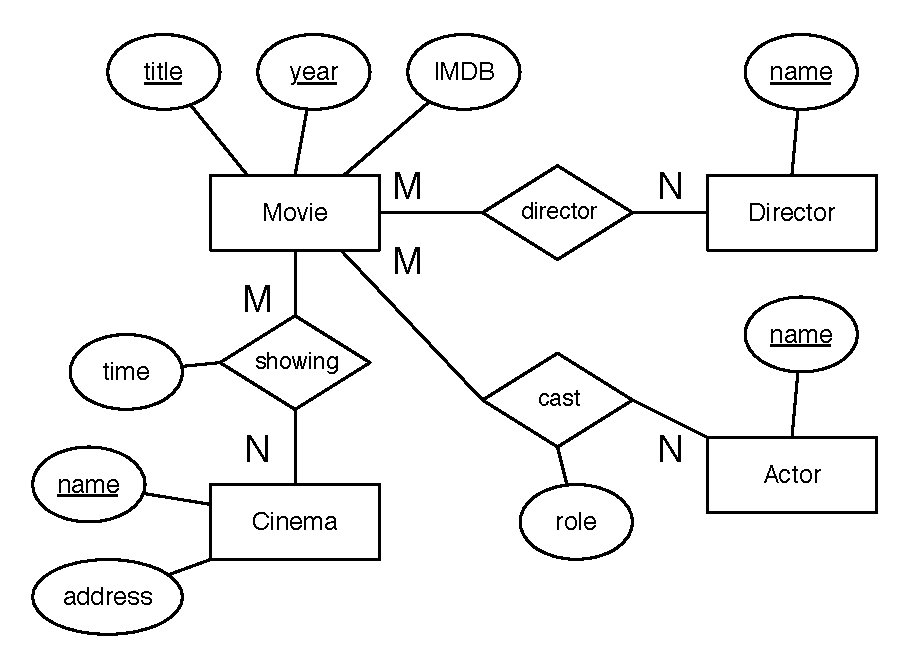
\includegraphics[width=\textwidth]{./figures/Movies_ER}
\end{column}
\end{columns}

\vskip0.5em

Must handle remakes (i.e., newer movie with the same title of an old one), and record IMDB scores (0 to 10) for the movies\footnote{A better design would be to also record the date when the IMDB score was collected, as they changes over time.}.

\end{frame}


\begin{frame}[fragile]
\label{schema1}
\vskip1em
\scalebox{0.9}{\usebox{\FullMovieSchema}}
\end{frame}

\begin{frame}[fragile]

In CMPUT291 you learned about \alert{schema refinement} by \textbf{normalization}, through decomposing relations that did not conform with a normal form.

\begin{itemize}[-, noitemsep, topsep=-5pt]
\item Normalization removes the chance of many update anomalies (which can cause many data inconsistencies). 
\item However, decomposing a ``conceptual'' relation into several smaller ones means we often need to \textbf{join} them back together to answer user queries.
\end{itemize}

\vskip1em 

In some applications, the extra cost of the joins might be unacceptable, in which case the schema is de-normalized for performance reasons.

\end{frame}

\begin{frame}

In CMPUT391 we will use a de-normalized, but simpler schema, where we represent the relationship \lstinline{Movie}--\lstinline{Director} as an attribute of \lstinline{Movie}, we eliminate the need for joins:

\vskip0.5em

\begin{center}
\hspace*{-1em}\fbox{\usebox{\SimplifiedMovieTableDDL}} % create table Movie
\end{center}

\vskip0.5em

\alert{PROS:} querying for movie directors is faster... \alert{CONS:} can't record movies with multiple directors; and directors disappear from the database if we delete their movies.
\end{frame}

\begin{frame}[fragile]
\label{schema2}

\underline{Simplified schema} used in the examples

\scalebox{0.9}{\usebox{\SimplifiedMovieSchema}}
\end{frame}



\begin{frame}[fragile]{Querying}

In CMPUT 291 you focused on translating \textbf{user/application needs} like ``who are the actors in movies directed by Debra Granik rated 7 or higher on IMDB?''

\vskip1em

Into \textbf{SQL}:

\begin{lstlisting}[style=SQL]
SELECT c.actor
FROM Cast c, Movie m
WHERE c.title=m.title AND c.year = m.year AND
      m.director = 'Debra Granik' AND m.IMDB >= 7;
\end{lstlisting}

\vskip1em

In 391 we care only about \textbf{how} to execute queries fast.

\end{frame}

%%%%%%%%%%% 391


\begin{frame}
\begin{center}
{\fontsize{26}{42}\selectfont What is CMPUT391 about? }

\vskip2em

\end{center}

\begin{columns}[onlytextwidth]
\begin{column}{0.475\textwidth}
\begin{BOX}{How is data stored?}
 - Hardware and I/O \\
 - heap and sequential files\\
 - index and hash files
\end{BOX}
\vskip1em
\begin{BOX}{SQL}
 - embedded SQL in C\\
 - recursion\\
 - triggers
\end{BOX}

\end{column}
\begin{column}{0.475\textwidth}
\begin{BOX}{Query processing?}
 - what does an \alert{algorithm} to perform a join look like? \\
 - what is its \alert{cost}?
\end{BOX}
\vskip1em
\begin{BOX}{Transactions?}
 - database logging\\
 - ACID transactions \\
 - Concurrency control
\end{BOX}

\end{column}
\end{columns}

All of that in single computer or distributed/parallel computer settings.

\end{frame}


\begin{frame}{How do we look at a database in 391?}

The schema (normalized or not) goes way.

We look at the files that store data (i.e., tables) and files that help us get to the data fast (i.e., indexes).

\vskip2em

\begin{tikzpicture}
\node [anchor=north west] at (-0.15,0) {\scalebox{0.85}{\usebox\TitleYearIndexOnMovie}} ;
\end{tikzpicture}

\end{frame}


\begin{frame}{What about queries and SQL updates?}

We want to understand what is the \alert{most efficient} way to execute them, keeping in mind:

\begin{enumerate}[label=(\alph*)]
\item data is kept in secondary memory and must be brought into memory before anything can be done to them;

\item the most efficient way of processing a statement depends both on \emph{static factors} (e.g., data organization) and \emph{dynamic factors} (e.g., the system load);

\item the DBMS \textbf{must support} multiple users/applications reading/writing the same database \textbf{concurrently}

\item the DBMS \textbf{must protect} the data from system failures, and \alert{ensure the database remains \textbf{consistent}} after each update
\end{enumerate}
\end{frame}

\begin{frame}{What \alert{else} is covered in CMPUT 391?}

\begin{enumerate}[label=\arabic* - ]
	\item Advanced relational constraints (aka Business Rules or Triggers)
	\item Advanced SQL (recursion, crisp semantics and evaluation algorithms)
	\item Non-relational data models and queries
		\begin{enumerate}[label=\roman* - ]
		\item RDF and SPARQL (\textbf{on your own} -- homework)
		\item XML and XQuery
		\item JSON and JSONiq (\textbf{on your own} -- homework)
		\item Spatial data and Nearest Neighbor queries (\textbf{on your own} -- coding asisgnments)
	\end{enumerate}
\end{enumerate}


\end{frame}



\begin{frame}{Prerequisites}

Prerequisite material which you are \highlight{expected to know} and will be tested on:

\vskip1em

\begin{block}{\alert{CMPUT 291}}
 - the relational model, SQL (DDL and DML) and the algebra\\
 - writing queries and translating between the algebra and SQL
\end{block}

\vskip1em

\begin{block}{\alert{CMPUT 201}}
- C programming; compiling and debugging C programs\\
- working with the command line and large files; git
\end{block}

\vskip1em

\begin{block}{\alert{CMPUT 204}}
- algorithms and data structures (e.g., linked lists, sorting, hashing)\\
- estimating time and space costs (e.g., $O(1)$, $O(n)$, $O(\log n)$).
\end{block}

\end{frame}

\begin{frame}{Common student complaints -- and the truth behind them}

\begin{enumerate}[label=\arabic* - ]
\item not enough time to do the assignments -- \alert{you have at least 3 weeks for each assignment}

\item \textbf{too much reading} -- \alert{no comment}

\item \textbf{we are supposed to learn things on our own} -- \alert{no comment}

\item no part marks for ``getting the idea right'' -- \alert{no reasonable answer is turned down in 391}

\item assignments are not worth enough -- \alert{they are there for you to practice and learn; plus \textbf{you will be tested on then in the exams}}

\item exams cover material not taught in class -- \alert{\textbf{yes they do}! homework and assignments are covered in the exams.}
\end{enumerate}


\end{frame}


\begin{frame}{Plagiarism -- what you should know}

\alert{\textbf{Every single case of plagiarism in CMPUT391 will be reported to the Faculty of Science.}}

\vskip1em

In previous academic terms sanctions were applied by the Faculty in every case reported. 

Most cases resulted in at least one letter grade reduction.

Repeating offenders received reductions of \alert{3 letter grades}.

Students have failed CMPUT391 because of cheating.
\end{frame}

\begin{frame}{How to succeed in CMPUT391?}

\begin{enumerate}[label=(\arabic*)]

\item Start early on the homework. They do take a lot of time.

\item \alert{\textbf{Consult a}} database \textbf{systems} \alert{book} regularly. Some slides condense many pages of material that cannot be explained in detail in class.

\item Read the supplemental material referenced from the slides.

\item \alert{Answer the practice questions} on your own. Most exam questions will be very similar to them.

\item Consult your TA regularly; ask them to help you with the practice questions.
\end{enumerate}

\end{frame}



\end{document}